%%%%%%%%%%%%%%%%%%%%%%%%%%%
% Este documento faz parte da classe cls-PFC-COEEL.cls
% NÃO ALTERE NENHUM DADO AQUI.
%%%%%%%%%%%%%%%%%%%%%%%%%%%
\pagestyle{EstiloPFC} % Estilo de página criado para o PFC do IFBA VDC
%%%% numeração da página em romano 
\pagenumbering{roman} 
%%%% espaçamento 1,5 entre linhas
\onehalfspacing
%%%%%%%%%%%%%%%%%%%%%%%%%%%%
%%%% CAPA 
%
% se é PFC faz capa de PFC

\ifbool{pfc}{
    \CapaPFC
}{}
    
% se é Relatório faz capa de Relatório
\ifbool{relatorio}{
    \CapaREL
}{}
%
%%%%%%%%%%%%%%%%%%%%%%%%%%%%
%%%% FOLHA DE ROSTO
% apenas para PFC
%
\ifbool{pfc}{ % se é PFC
    \newpage\clearpage\pagebreak
    \ifpdf\phantomsection\fi
    \addcontentsline{toc}{chapter}{Folha de Rosto}
    \FolhaRosto%
}{}
%
%%%%%%%%%%%%%%%%%%%%%%%%%%%%
%%%% FICHA CATALOGRÁFICA
% apenas para PFC
%
\ifbool{pfc}{ % se é PFC
    \newpage\clearpage\pagebreak
    \ifpdf\phantomsection\fi
    \addcontentsline{toc}{chapter}{Ficha Catalográfica}
    % inclua o PDF da ficha catalográfica feita pela biblioteca
    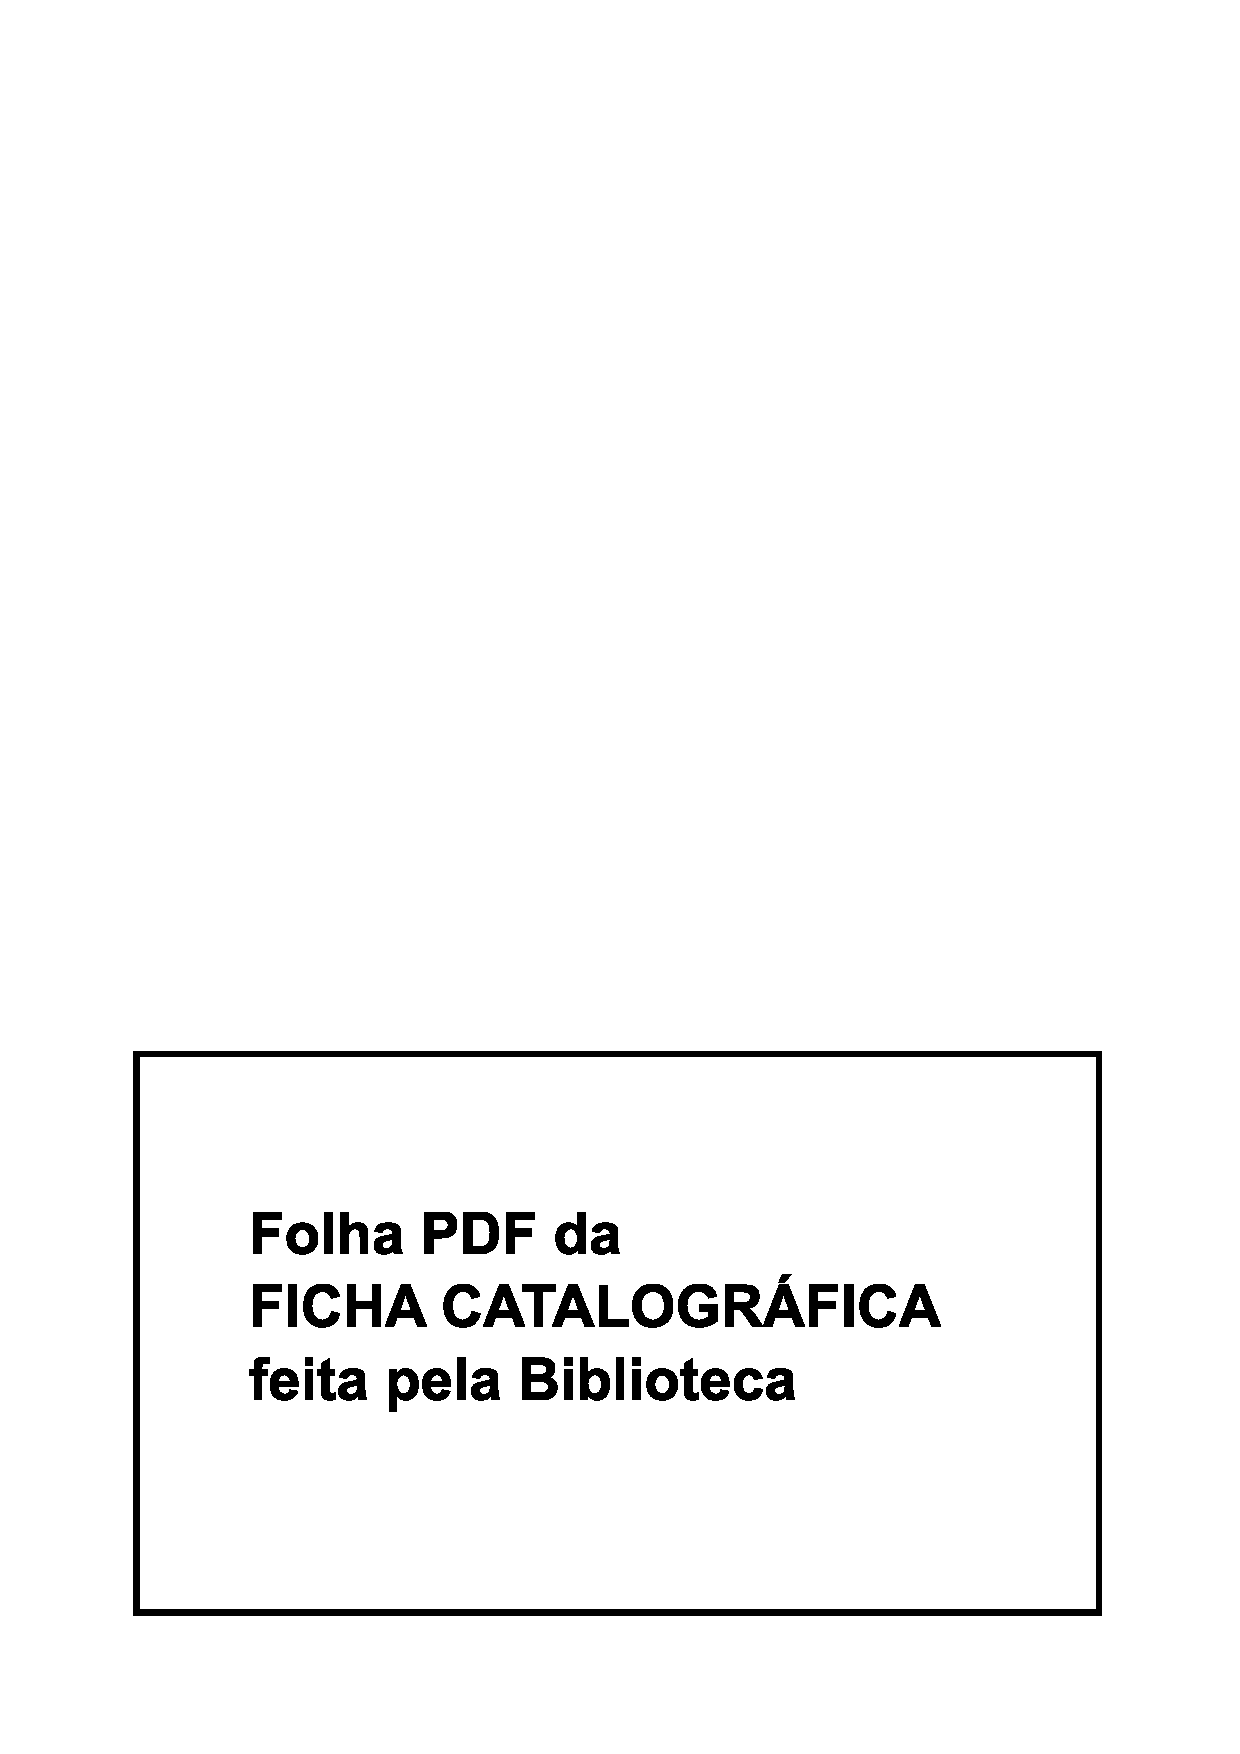
\includepdf[pages=1]{./PFC_Especificos/Ficha_Catalografica.pdf}
}{}
%
%%%%%%%%%%%%%%%%%%%%%%%%%%%%
%%%% FOLHA DE APROVAÇÃO
% Apenas para PFC
%
\ifbool{pfc}{ % se é PFC
    \newpage\clearpage
    \ifpdf\phantomsection\fi
    \addcontentsline{toc}{chapter}{Folha de Aprovação}
    
    % inclua o PDF da folha de aprovação assinada digitalmente pelos membros da banca pelo SEI ou pelo SOU.GOV:

    % \includepdf[pages=1]{Folha_Aprovacao.pdf} % descomente esta linha quando for anexar o PDF

    % comente esta linha quando for anexar o PDF
    %%%%%%%%%%%%%%%%%%%%%%%%%%%%%%%%%%%%%%%%%%%%%
%%%%%% FOLHA DE APROVAÇÃO
%%%%%%%%%%%%%%%%%%%%%%%%%%%%%%%%%%%%%%%%%%%%%

% caso queira incluir o PDF da folha de aprovação assinada digitalmente pelos membros da banca pelo SEI ou pelo SOU.GOV, acrescente o arquivo PDF utilizando o comando seguinte comando dentro do arquivo MAIN:
% \includepdf[pages=1]{Folha_Aprovacao.pdf} % descomente esta linha se for anexar o PDF

  \clearpage\newpage\pagebreak%
  \pagestyle{plain}
  \begin{center}%
    \textbf{\Large \@Titulo  }\\%
    \vspace{1.2cm}%
    \MakeUppercase{\textbf{\Large \@Autor}}\\%
  \end{center}%
  \vspace{0.6cm}%

  A presente Monografia, apresentada em sessão realizada em \textbf{ \@DataDefesa}, foi avaliada como adequada para a obtenção do Grau de Bacharel em Sistemas de Informação, julgada \textbf{aprovada} em sua forma final pela Coordenação do Curso de Sistemas de Informação do Instituto Federal de Educação, Ciência e Tecnologia da Bahia, \textit{campus} Vitória da Conquista.

  \begin{center}
    
    \vspace{7mm}
    Vitória da Conquista/BA, \@DataDefesa.
    \vspace{7mm}
    \vspace{7mm}
    \rule[0cm]{10cm}{0,5mm}\\
    \textbf{}
    Prof. Me. Alexandro dos Aantos Silva\\
    (Coordenador do Curso - IFBA campus Vitória da Conquista)\\
    \vspace{7mm}
    \textbf{\small BANCA EXAMINADORA:}\par
    \vspace{7mm}
    \rule[0cm]{10cm}{0,5mm}\\
    Prof. DSc. Djan Almeida Santos (Orientador)\\
    IFBA campus Vitória da Conquista\\
    \vspace{7mm}
    \rule[0cm]{10cm}{0,5mm}\\
    Prof. Msc. Crijina Chagas Flores\\
    IFBA campus Vitória da Conquista\\

    \vspace{7mm}
    \rule[0cm]{10cm}{0,5mm}\\
    Prof. Msc. Liojes de Oliveira Carneiro\\
    IFBA campus Vitória da Conquista\\
    
  \end{center}
  
  
  % \vfill % leva para o botton da página
  % \begin{center}%    
  %   {\large  \@CidadeDefesa}\\%
  %   \vspace{1mm}%
  %   {\large  \@DataDefesa }%
  % \end{center}%
 
}{}
%
%%%%%%%%%%%%%%%%%%%%%%%%%%%
%%%% DEDICATÓRIA
% Apenas para PFC
%
\ifbool{pfc}{ % se é PFC
    \newpage\clearpage\pagebreak
\pagestyle{plain}
~\vfill
\begin{flushright}
    % Aqui vai a Dedicatória de seu PFC
    \textit{Dedico esta obra à Deus, aos meus professores e à minha família, dedico também \ldots} \\

    \vspace{1cm}
    \textit{O que faz andar o barco não é a vela enfunada, mas o vento que não se vê.~
[Platão]}
\end{flushright}


}{}
%
%%%%%%%%%%%%%%%%%%%%%%%%%%%%
%%%% AGRADECIMANTOS
% Apenas para PFC
%
\ifbool{pfc}{ % se é PFC
    \pagebreak\newpage\clearpage
\pagestyle{plain}

\chapter*{AGRADECIMENTOS}
    % Aqui vão os agradecimentos de seu PFC
    Agradeço este trabalho ao IFBA pelo ensino de qualidade com ótimos professores, e ao meu orientador pelo empenho, dedicação e parceria. Agradeço também \ldots

}{}
%
%%%%%%%%%%%%%%%%%%%%%%%%%%%%
%%%% RESUMO
% Apenas para PFC
%
\ifbool{pfc}{ % se é PFC
    \newpage\clearpage
    \ifpdf\phantomsection\fi
    \addcontentsline{toc}{chapter}{Resumo}
    \clearpage\newpage\pagebreak%
\pagestyle{plain}

\Resumo 
Este trabalho descreve o desenvolvimento da plataforma web {\bf MeuPetAqui}, uma rede social para donos de animais de estimação e Organizações Não Gorvenamentais (\gls{ONGs}) envolvidas na proteção animal. A plataforma permite a criação de postagens, conexão entre usuários, promoção da adoção, busca por tutores de animais encontrados e auxílio no rastreamento de animais perdidos. Além disso, inclui ferramentas como o Registro Geral Animal (\gls{RGA}) para identificação do pet e de seu tutor, e o controle de vacinação, facilitando a gestão de vacinas e medicamentos recebidos pelo animal. A plataforma também atua como meio de divulgação de campanhas de arrecadação de recursos para tratamento de animais cuidados pelas ONGs.

A plataforma é utilizada por dois tipos de usuários: usuários comuns, que podem criar postagens, perfis para seus animais de estimação e emitir alertas relacionados à adoção, pets encontrados ou perdidos; e ONGs, que possuem as mesmas funcionalidades, além de alertas para animais que necessitam de cuidados veterinários. Os posts são exibidos na timeline principal, enquanto uma segunda timeline é dedicada exclusivamente aos alertas, destacando a importância da conscientização e do engajamento em causas do bem-estar animal.

O trabalho aborda a criação de um sistema que promove a conscientização e engajamento em questões relacionadas ao bem-estar animal. A plataforma MeuPetAqui é uma ferramenta para conectar simpatizantes da causa, proprietários de animais de estimação e ONGs, contribuindo para a redução do número de animais abandonados e promovendo relacionamentos saudáveis entre donos e seus animais de estimação.
%{\bf Título}
% máximo de 6 palavras chave separadas por vírgula
\begin{keywords}
plataforma web, MeuPetAqui, rede social, animais de estimação, rastreamento,ONGs
\end{keywords}
}{}
%
%%%%%%%%%%%%%%%%%%%%%%%%%%%%
%%%% ABSTRACT
% Apenas para PFC
%
\ifbool{pfc}{ % se é PFC
    \newpage\clearpage
    \ifpdf\phantomsection\fi
    \addcontentsline{toc}{chapter}{Abstract}
    \clearpage\newpage\pagebreak%
\pagestyle{plain}

\Abstract

This work describes the development of the web platform {\bf MeuPetAqui}, a social network for pet owners and animal protection non-governmental organizations (\gls{NGOs}). The platform allows users to create posts, connect with others, promote adoption, search for owners of found animals, and assist in tracking lost animals. It also includes features such as the General Animal Registry (\gls{RGA}) for pet and owner identification, as well as vaccination control to facilitate management of vaccines and medications received by the animal. The platform also serves as a means of promoting fundraising campaigns for the treatment of animals cared for by NGOs.

The platform is used by two types of users: regular users, who can create posts, profiles for their pets, and issue alerts related to adoption, found or lost pets; and NGOs, who have the same functionalities, as well as alerts for animals in need of veterinary care. User posts and their friends' posts are displayed in the main timeline, while a second timeline is dedicated exclusively to alerts, emphasizing the importance of raising awareness and engaging in animal welfare causes.

This work addresses the creation of a system that promotes awareness and engagement in animal welfare issues. The MeuPetAqui platform is a valuable tool for connecting sympathizers of the cause, pet owners, and NGOs, actively contributing to reducing the number of abandoned animals and fostering healthy relationships between owners and their pets.

\begin{keywords}
web platform, MeuPetAqui, social network, pets, tracking, NGOs
\end{keywords}
}{}
%


%%%%%%%%%%%%%%%%%%%%%%%%%%%%
%%%% LISTA DE FIGURAS
% Apenas para PFC
%
\ifbool{pfc}{ % se é PFC
    \newpage\clearpage
    \ifpdf\phantomsection\fi
    \addcontentsline{toc}{chapter}{\listfigurename}
    \listoffigures
}{}
%
%%%%%%%%%%%%%%%%%%%%%%%%%%%%
%%%% LISTA DE TABELAS
% Apenas para PFC
%
\ifbool{pfc}{ % se é PFC
    \clearpage\newpage
    \ifpdf\phantomsection\fi
    \addcontentsline{toc}{chapter}{\listtablename}
    \listoftables
}{}
%
%%%%%%%%%%%%%%%%%%%%%%%%%%%%
%%%% LISTA DE CÓDIGOS
%
% Apenas para PFC
%
\ifbool{pfc}{ % se é PFC
    \clearpage\newpage
    \newcommand{\lstlistoflistingsname}{Lista de Códigos}
    \renewcommand{\lstlistingname}{Código}
    \addcontentsline{toc}{chapter}{Lista de Códigos\numberline{}}
    \lstlistoflistings
}{}
%
%%%%%%%%%%%%%%%%%%%%%%%%%%%%
%%%% GLOSSÁRIO
%%%% LISTA DE SÍMBOLOS E SIGLAS
%
% https://pt.overleaf.com/learn/latex/Glossaries
%
% Apenas para PFC
%
\ifbool{pfc}{ % se é PFC
    \clearpage\newpage\pagebreak
    \renewcommand{\glossaryname}{Glossário: Símbolos e Siglas}
    \addcontentsline{toc}{chapter}{\glossaryname}
    \renewcommand{\pagelistname}{Páginas}%
    \printglossary[style=long3col-booktabs]
}{}
%
%%%%%%%%%%%%%%%%%%%%%%%%%%%%
%%%% SUMÁRIO
%
% Apenas para PFC
%
\ifbool{pfc}{ % se é PFC
    \clearpage\pagebreak\newpage
    \renewcommand{\cftchapleader}{\cftdotfill{\cftdotsep}} % capítulos do sumário com linha de pontos
    \tableofcontents
}{}
%
%%%%%%%%%%%%%%%%%%%%%%%%%%%%
%
\pagestyle{EstiloPFC} % estilo criado para este PFC
\clearpage\pagebreak\newpage
\onehalfspacing % espaçamento 1,5 entre linhas
\pagenumbering{arabic}  % numeração das páginas em algarismos arábicos
\makeatother %  restringir o uso do símbolo @ em comandos de macro
%
%%%%%%%%%%%%%%%%%%%%%%%%%%%%